%%%%%%%%%%%%%%%%%%%%%%%%%%%%%%%%%%%%%%%%%
% a0poster Portrait Poster
% LaTeX Template
% Version 1.0 (22/06/13)
%
% The a0poster class was created by:
% Gerlinde Kettl and Matthias Weiser (tex@kettl.de)
% 
% This template has been downloaded from:
% http://www.LaTeXTemplates.com
%
% License:
% CC BY-NC-SA 3.0 (http://creativecommons.org/licenses/by-nc-sa/3.0/)
%
%%%%%%%%%%%%%%%%%%%%%%%%%%%%%%%%%%%%%%%%%

%----------------------------------------------------------------------------------------
%	PACKAGES AND OTHER DOCUMENT CONFIGURATIONS
%----------------------------------------------------------------------------------------

\documentclass[a0,portrait]{a0poster}

\usepackage{multicol} % This is so we can have multiple columns of text side-by-side
\columnsep=100pt % This is the amount of white space between the columns in the poster
\columnseprule=3pt % This is the thickness of the black line between the columns in the poster

\usepackage[svgnames]{xcolor} % Specify colors by their 'svgnames', for a full list of all colors available see here: http://www.latextemplates.com/svgnames-colors

\usepackage{times} % Use the times font
%\usepackage{palatino} % Uncomment to use the Palatino font

\usepackage{graphicx} % Required for including images
\graphicspath{{figures/}} % Location of the graphics files
\usepackage{booktabs} % Top and bottom rules for table
\usepackage[font=small,labelfont=bf]{caption} % Required for specifying captions to tables and figures
\usepackage{amsfonts, amsmath, amsthm, amssymb, enumitem} % For math fonts, symbols and environments
\usepackage{wrapfig} % Allows wrapping text around tables and figures

\usepackage{tcolorbox}

\begin{document}
\pagecolor{white!90!black}
%----------------------------------------------------------------------------------------
%	POSTER HEADER 
%----------------------------------------------------------------------------------------

% The header is divided into two boxes:
% The first is 75% wide and houses the title, subtitle, names, university/organization and contact information
% The second is 25% wide and houses a logo for your university/organization or a photo of you
% The widths of these boxes can be easily edited to accommodate your content as you see fit

\begin{minipage}[b]{0.75\linewidth}
\veryHuge \color{NavyBlue} \textbf{Optimal design of experiment:} \color{Black}\\ % Title
\Huge\textit{supercritical fluid extraction case}\\[2cm] % Subtitle
\huge \textbf{Oliwer Sliczniuk, Pekka Oinas}\\[0.5cm] % Author(s)
\huge School of Chemical Engineering, Aalto University, Finland\\[0.4cm] % University/organization
%\Large \texttt{john@LaTeXTemplates.com} --- 1 (000) 111 1111\\
\end{minipage}
%
\begin{minipage}[b]{0.25\linewidth}

\includegraphics[width=15cm]{Aalto_University_logo.png}\\ \\
\end{minipage}

%\vspace{0.5cm} % A bit of extra whitespace between the header and poster content
\noindent\rule{\textwidth}{3pt}
%\vspace{0.25cm} % A bit of extra whitespace between the header and poster content

%----------------------------------------------------------------------------------------

\begin{multicols}{2} % This is how many columns your poster will be broken into, a portrait poster is generally split into 2 columns

%----------------------------------------------------------------------------------------
%	ABSTRACT
%----------------------------------------------------------------------------------------

%\color{Navy} % Navy color for the abstract

%\begin{abstract}

%\end{abstract}

%----------------------------------------------------------------------------------------
%	INTRODUCTION
%----------------------------------------------------------------------------------------

%\color{Navy} % SaddleBrown color for the introduction

\begin{tcolorbox}[width=\linewidth, boxrule=0mm, sharp corners=all, colback=white]
	{\LARGE Introduction\\}

This study investigates the extraction of essential oils from chamomile flowers using supercritical carbon dioxide as a solvent in a semi-batch mode. The process is described by a mathematical model incorporating empirical correlations. The goal of this work is to \underline{improve the precision of the} \underline{model parameters by designing a new experiment} and validating the model against it.
\end{tcolorbox}

%----------------------------------------------------------------------------------------
%	OBJECTIVES
%----------------------------------------------------------------------------------------

%\color{DarkSlateGray} % DarkSlateGray color for the rest of the content

%\section*{Main Objectives}

%\begin{enumerate}
%\item Lorem ipsum dolor sit amet, consectetur.
%\item Nullam at mi nisl. Vestibulum est purus, ultricies cursus volutpat sit amet, vestibulum eu.
%\item Praesent tortor libero, vulputate quis elementum a, iaculis.
%\item Phasellus a quam mauris, non varius mauris. Fusce tristique, enim tempor varius porta, elit purus commodo velit, pretium mattis ligula nisl nec ante.
%\item Ut adipiscing accumsan sapien, sit amet pretium.
%\item Estibulum est purus, ultricies cursus volutpat
%\item Nullam at mi nisl. Vestibulum est purus, ultricies cursus volutpat sit amet, vestibulum eu.
%\item Praesent tortor libero, vulputate quis elementum a, iaculis.
%\end{enumerate}

%----------------------------------------------------------------------------------------
%	MATERIALS AND METHODS
%----------------------------------------------------------------------------------------

%\section*{Materials and Methods}

%Fusce magna risus, molestie ut porttitor in, consectetur sed mi. Vestibulum ante ipsum primis in faucibus orci luctus et ultrices posuere cubilia Curae; Pellentesque consectetur blandit pellentesque. Sed odio justo, viverra nec porttitor vel, lacinia a nunc. Suspendisse pulvinar euismod arcu, sit amet accumsan enim fermentum quis. In id mauris ut dui feugiat egestas. Vestibulum ac turpis lacinia nisl commodo sagittis eget sit amet sapien.

%------------------------------------------------

%\section*{Process Model}
\begin{tcolorbox}[width=\linewidth, boxrule=0mm, sharp corners=all, colback=white]
	{\LARGE Process Model\\}
	
	The process is described by a first-principle distributed-parameter model [1,2] with a set of empirical correlations [2]. The model assumptions are \\

\begin{minipage}[b]{0.5\linewidth}
	\begin{itemize}
		\item One-dimensional
		\item Plug flow
		\item No pressure drop
		\item Uniform particle distribution
	\end{itemize}
\end{minipage}
\hfill
\begin{minipage}[b]{0.5\linewidth}
	\begin{itemize}
		\item Two-film theory for a single component
		\item Peng-Robinson equation of state
		\item Decaying extraction kinetic
		\item Empirical correlations
	\end{itemize}
\end{minipage}

%\begin{minipage}[b]{0.5\linewidth}
%	\begin{itemize}
%		\item Based on the two-film theory for a single component
%		\item Peng-Robinson equation of state
%		\item Decaying extraction kinetic
%		\item Empirical correlations
%	\end{itemize}
%\end{minipage}

%The extraction process is represented by a \underline{distributed-parameter model} consisting of partial differential equations. This model has been validated within the operating conditions: temperatures between $30 - 40^\circ C$, pressures between $100 - 200$ bar, and mass flow rates between $3.33 - 6.67 \times 10^{-5}$ kg/s. The solute extraction from the solid to the fluid phase is described using the two-film theory for a single component. The physical properties of the fluid and pseudo-homogeneous phase are considered to be locally dependent on temperature and pressure and are calculated using the Peng-Robinson equation of state. By incorporating the enthalpy balance, the extraction kinetic becomes a function of operating conditions. Empirical correlations were developed to generalize the process model across the entire range of operating conditions.

\begin{align*}
	\dot{x} = \cfrac{d x}{d t} = 
	\begin{bmatrix}
		\frac{\partial c_f}{\partial t} \\
		\\
		\cfrac{\partial c_s}{\partial t} \\
		\\
		\cfrac{\partial \left(\rho_f h A_f\right)}{\partial t} \\
		\\
		\cfrac{d y}{d t}
	\end{bmatrix}
	=
\underbrace{\begin{bmatrix}
		-\frac{1}{\phi} \frac{\partial \left( c_f u\right)}{\partial z} - \frac{1-\phi}{\phi} \cfrac{\partial c_s}{\partial t} + \frac{1}{\phi} \frac{\partial}{\partial z} \left( D^M_e \frac{\partial c_f}{\partial z} \right) \\
		-\cfrac{ D_i^R \exp \left( \Upsilon \left( 1-\cfrac{ c_s }{c_{s0}} \right) \right) }{ \mu l^2 } \left( c_s  - \cfrac{\rho_s c_f }{ k_m \rho_f }  \right) \\
		- \cfrac{\partial \left( \rho_f h A_f {\color{red}v} \right)}{\partial z} + \cfrac{\partial \left(P A_f\right)}{\partial t} + \cfrac{\partial}{\partial z} \left( k \cfrac{\partial T}{\partial z} \right) \\
		\cfrac{F}{\rho_f} c_f \biggr\rvert_{z=L}
	\end{bmatrix}}_{G(x,t,\Theta;\Xi)}
\end{align*}

\begin{minipage}[h!]{0.33\linewidth}
	\begin{align*}
		c_f &- \text{Solutes concentration in the fluid phase}\\
		c_s &- \text{Solutes concentration in the solid phase}\\
		h~  &- \text{Enthalpy}\\
		y~ &- \text{Extraction yield}\\
		\rho_f &- \text{Density of fluid}\\
		A_f &- \text{Cross-section of the bed}\\
		u~~ &- \text{Darcy velocity}\\
		\phi~~ &- \text{Void fraction}\\
		D_e^M &- \text{Axial mass diffusivity}\\
		D_i^R &- \text{Internal mass diffusivity}
	\end{align*}
\end{minipage}
%
\begin{minipage}[h!]{0.33\linewidth}
	\begin{align*}
		\mu~ &- \text{Particle shape coefficient}\\
		l~ &- \text{Particle length}\\
		\Upsilon~ &- \text{Decaying factor}\\
		\rho_s &- \text{Bulk density of solid bed}\\
		k_m &- \text{Partition factor}\\
		P~ &- \text{Pressure}\\
		T~ &- \text{Temperature}\\
		F~ &- \text{Mass flow rate} \\
		\Sigma~ &- \text{Covariance matrix} \\
		\Theta~ &- \text{Vector of parameters}
	\end{align*}
\end{minipage}

\begin{center}\vspace{0.5cm}
	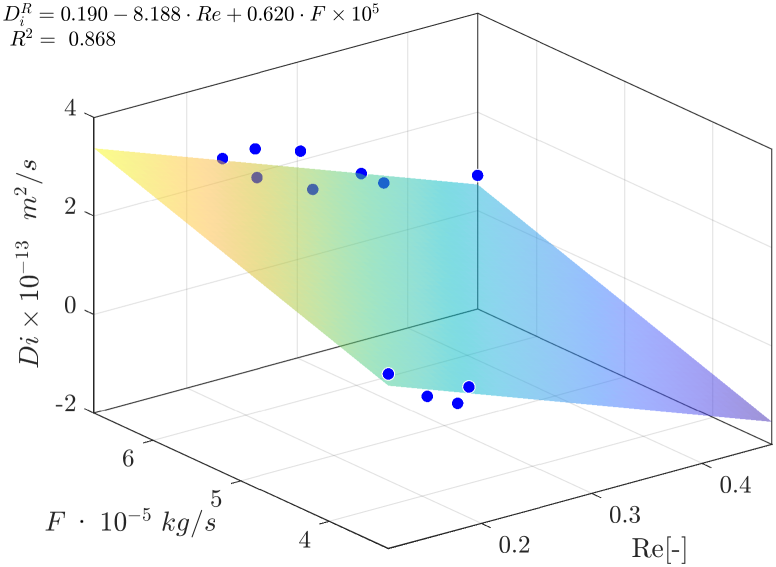
\includegraphics[width=0.49\linewidth]{Di_Re_F_1.png}
	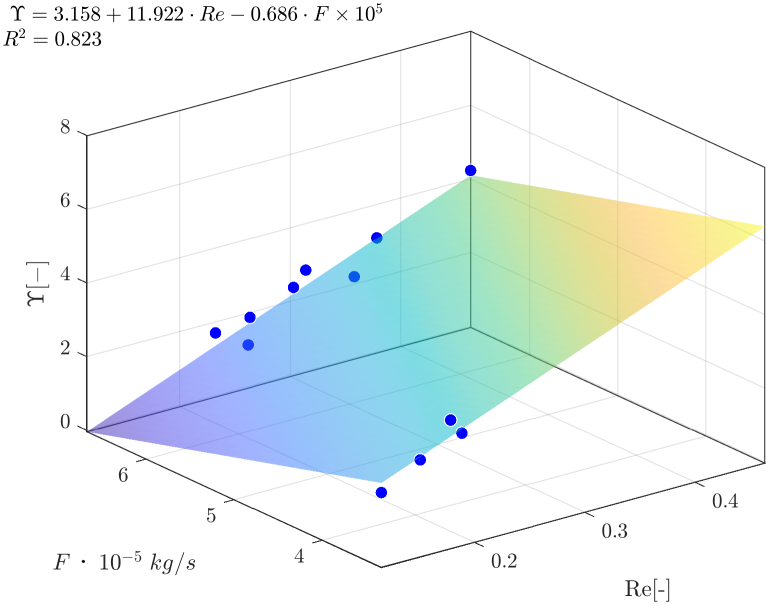
\includegraphics[width=0.49\linewidth]{Gamma_Re_F_1.png}
	\captionof{figure}{Empirical correlations}
\end{center}%\vspace{1cm}

\end{tcolorbox}

\begin{tcolorbox}[width=\linewidth, boxrule=0mm, sharp corners=all, colback=white]
%------------------------------------------------
%\vspace{1cm}
%\section*{Model-based optimal design of experiment}
\begin{tcolorbox}[width=\linewidth, boxrule=0mm, sharp corners=all, colback=white]
	{\LARGE Model-based optimal design of experiment\\}
\end{tcolorbox}

\underline{Fisher information $\mathcal{F}$ (Hessian of the likelihood function) measurs the amount of information} observable random variables carry about a parameters of a distribution that models these variables[3]:

\begin{equation*}
	%\Sigma^{-1} \geq
	\mathcal{F}(t,\Theta; \Xi) = \frac{\partial y(t, \Theta; \Xi)}{\partial \Theta} \Sigma \frac{\partial y(t, \Theta; \Xi)}{\partial \Theta^\top}
\end{equation*}

%The optimal design of experiments involves planning an experiment in such a way that parameters can be estimated without bias and with minimal variance. 
The D-optimality criterion is chosen as the objective function, aiming to \underline{minimize the volume} \underline{of the ellipsoidal confidence region of parameter estimates} under the experimental conditions $\Xi$.

\begin{equation*}
	\begin{aligned} 
		&\Xi^* &= \arg &\min_{ T^{in},~F\in~\Xi}\quad\int_{t_0}^{t_f} - \ln \det \mathcal{F}(t,\Theta; \Xi)~dt  \\
		&\text{subject to}
		& \dot{x} = ~&G~~(x,t,\Theta;\Xi) \\
		&& T^{0} = ~&T^{in}(t=0) \\
		&& 30^\circ C \leq ~&T^{in}(t) ~ \leq 40^\circ C \\
		&& 3.33 \cdot 10^{-5}~\text{kg/s} \leq ~&F~~(t)~ \leq 6.67 \cdot 10^{-5}~\text{kg/s}\\
		&& 100~\text{bar} \leq ~&P~~(t)~ \leq 200~\text{bar} \\
	\end{aligned}
\end{equation*}

This work aims \underline{to improve the precision of the correlation for $D_i^R$} by designing an experiment with dynamically changing operating conditions (\underline{$F$ and $T^{in}$)}. \\

The method of lines is employed to transform the process model equations into a set of ODEs. The first- and second-order derivatives are approximated using the backward and central difference schemes, respectively. The time integral and all time-dependent functions are discretized using the single-shooting approach with piecewise-constant controls to obtain a static non-linear program.
\end{tcolorbox}


%----------------------------------------------------------------------------------------
%	RESULTS 
%----------------------------------------------------------------------------------------
\begin{tcolorbox}[width=\linewidth, boxrule=0mm, sharp corners=all, colback=white]
	{\LARGE Results\\}
	
	The system operates for 300 minutes, with a sampling interval of 10 minutes and decision variables adjusted every 15 minutes. Each of the five analysed cases assumes a constant pressure, set at 100, 125, 150, 175, and 200 bar. To identify the global solution, the optimization problem is solved multiple times, each starting from a random initial solution sampled from a uniform distribution. %Figure 2 compares the initial and final values of the cost function across multiple optimization runs for different cases of pressure value.
	
	\begin{center}\vspace{0.5cm}
		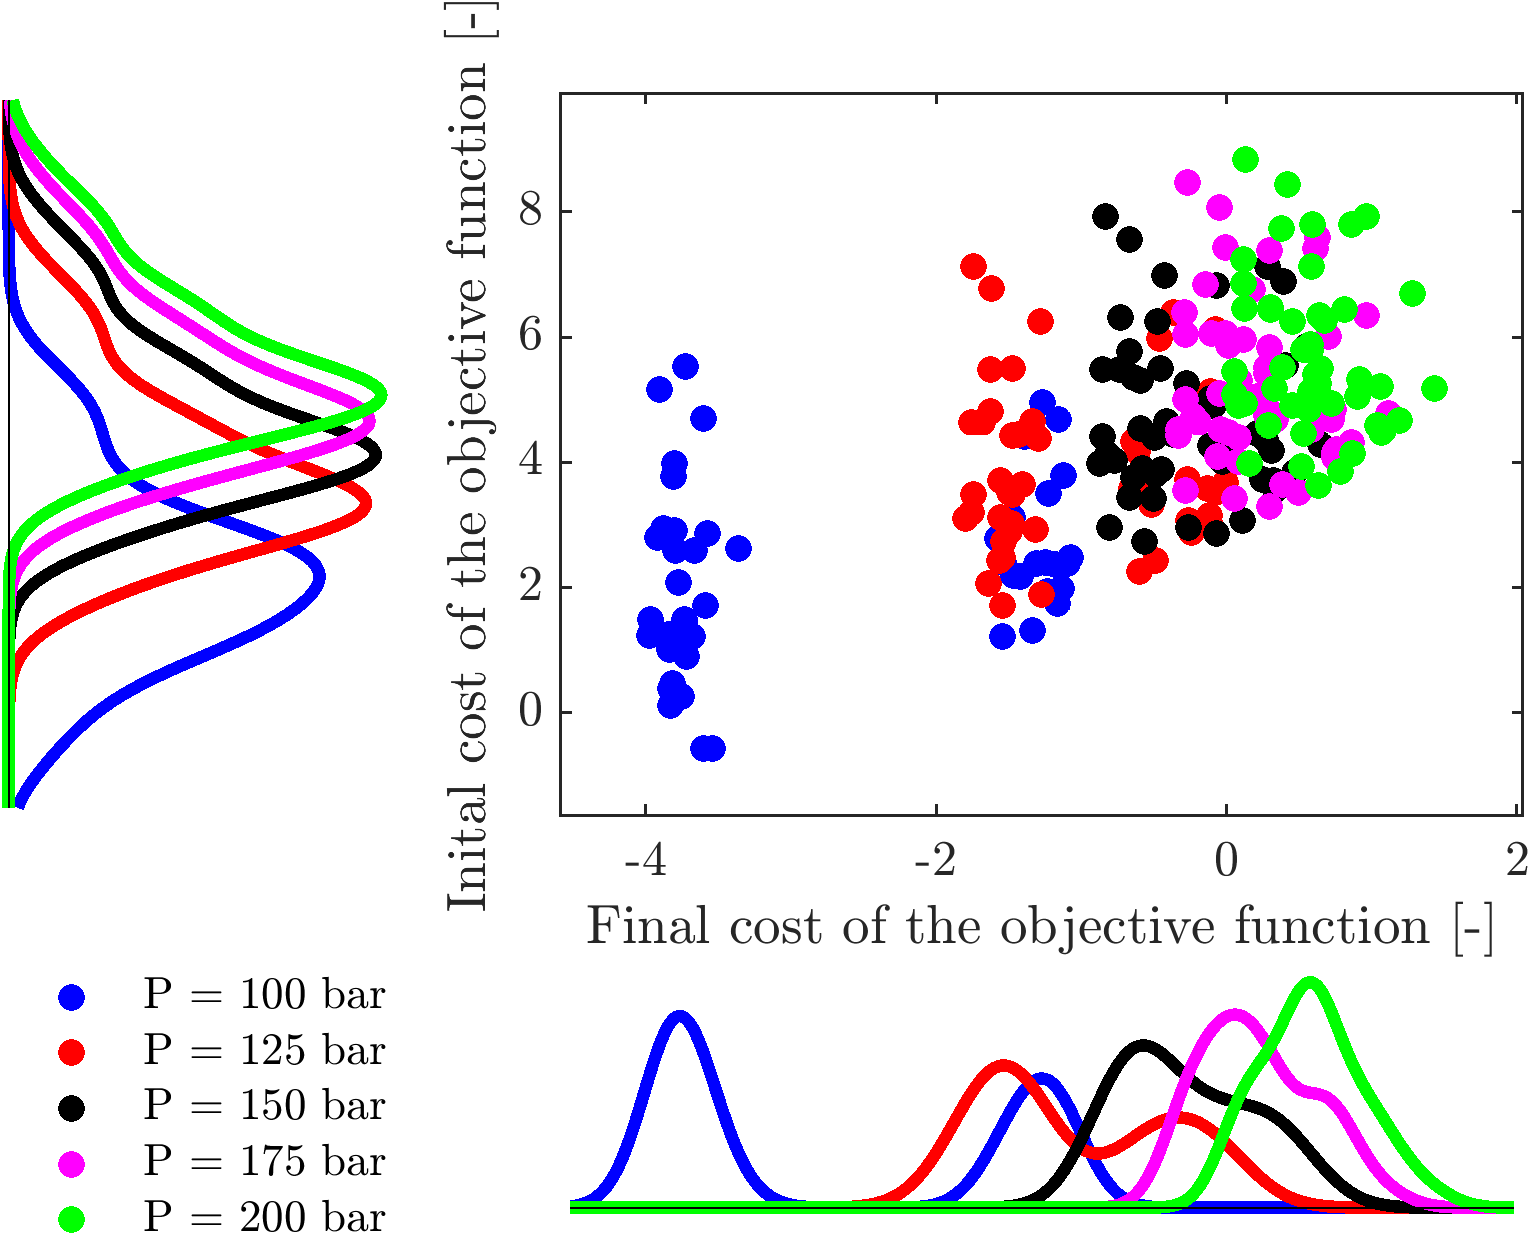
\includegraphics[width=\linewidth]{scatter.png}
		\captionof{figure}{Values of the objective function}
	\end{center}%\vspace{1cm}
	
	The optimal profiles of the inlet temperature and flow rates for each case are showed in Figure 3
	
	\begin{center}\vspace{0.5cm}
		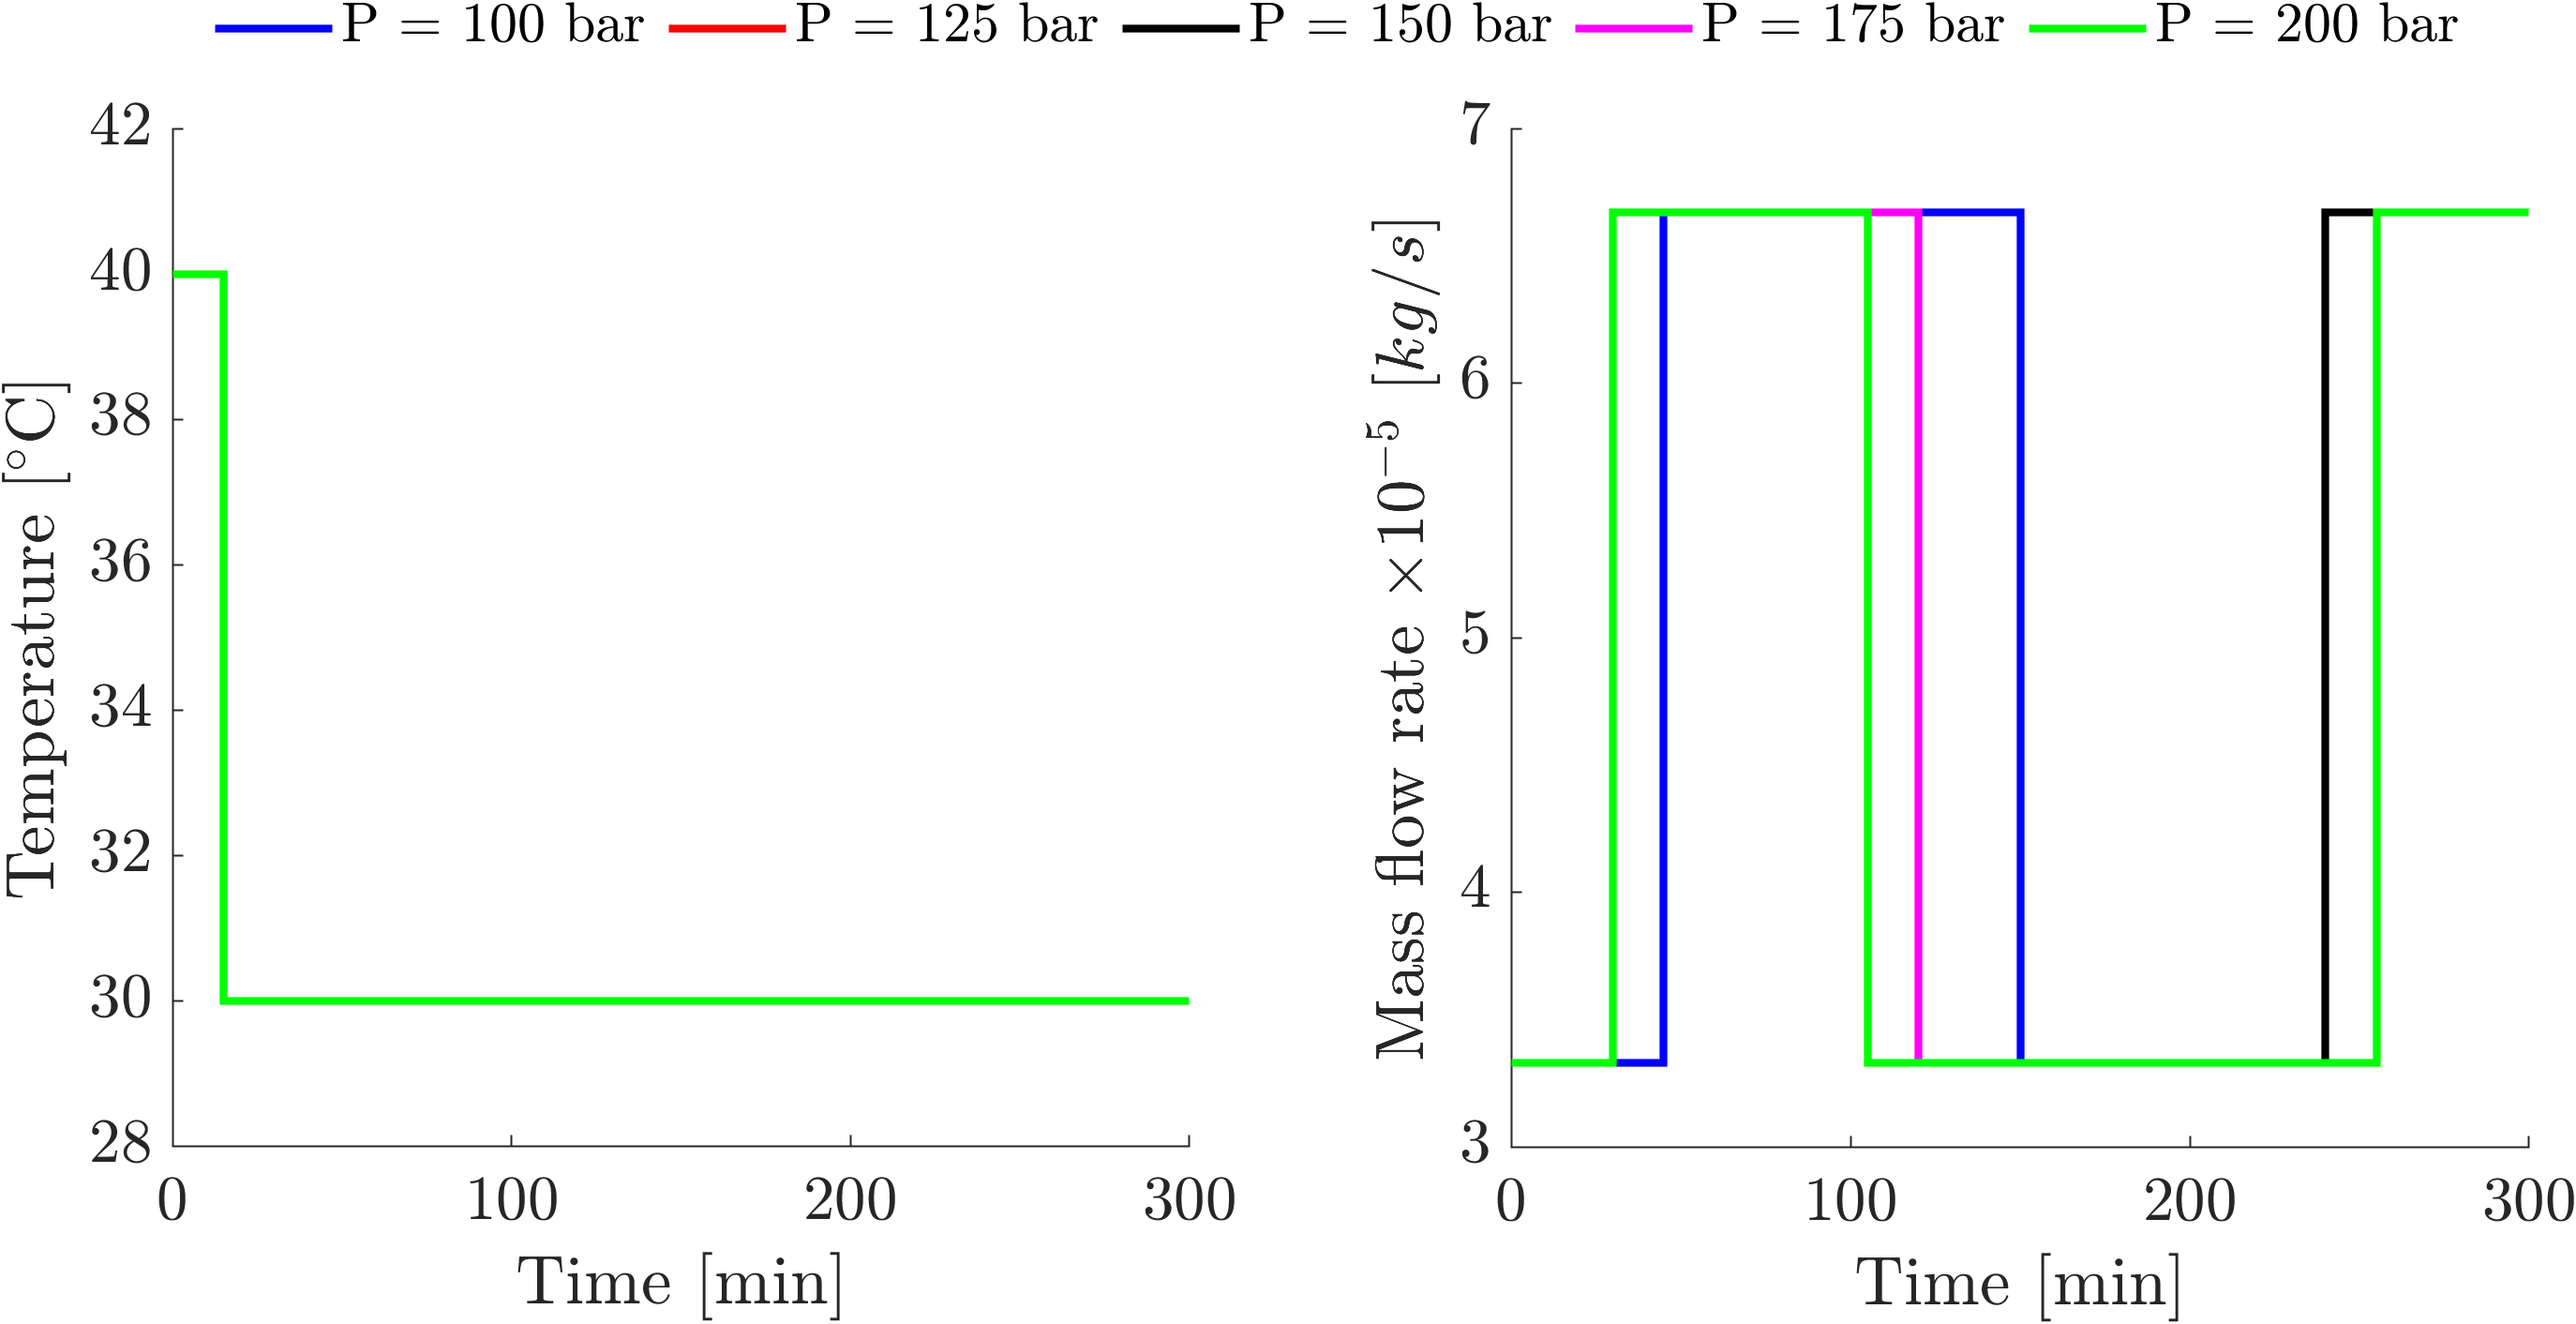
\includegraphics[width=\linewidth]{Profiles.png}
		\captionof{figure}{Optimal profiles}
	\end{center}%\vspace{1cm}
	
\end{tcolorbox}

%----------------------------------------------------------------------------------------
%	CONCLUSIONS
%----------------------------------------------------------------------------------------

\begin{tcolorbox}[width=\linewidth, boxrule=0mm, sharp corners=all, colback=white]
	{\LARGE Conclusions\\}

	\begin{itemize}
		\item The optimal control profiles are similar across all cases.
		\item Low objective values are achieved at pressures near the supercritical point, where variations in the inlet temperature cause significant deviations in the physical properties of CO$_2$ and consequently in the Reynolds number
		\item The mass flow rate is the primary control variable, indicating that the system is more sensitive to mass flow rate changes than to inlet temperature variations.
	\end{itemize}

\end{tcolorbox}

%----------------------------------------------------------------------------------------
%	FORTHCOMING RESEARCH
%----------------------------------------------------------------------------------------

%\section*{Forthcoming Research}

%Vivamus molestie, risus tempor vehicula mattis, libero arcu volutpat purus, sed blandit sem nibh eget turpis. Maecenas rutrum dui blandit lorem vulputate gravida. Praesent venenatis mi vel lorem tempor at varius diam sagittis. Nam eu leo id turpis interdum luctus a sed augue. Nam tellus.

 %----------------------------------------------------------------------------------------
%	REFERENCES
%----------------------------------------------------------------------------------------
\begin{tcolorbox}[width=\linewidth, boxrule=0mm, sharp corners=all, colback=white]
	{\LARGE References\\}
	\begin{enumerate}[label={[\arabic*]}]
		\item E. Reverchon. Mathematical modeling of supercritical extraction of sage oil. AIChE Journal, 42(6):1765–1771, June 1996. ISSN 1547-5905. doi: 10.1002/aic.690420627.
		\item O. Sliczniuk and P. Oinas. Supercritical fluid extraction of essential oil from chamomile flowers: modelling and parameter estimation. CJCE Journal. June 2024. Under review.
		\item E. Walter and L. Pronzato. Identification of parametric models from experimental data. Communications and control engineering. Springer, London, 2010. ISBN 9781849969963
	\end{enumerate}
\end{tcolorbox}
%----------------------------------------------------------------------------------------
%	ACKNOWLEDGEMENTS
%----------------------------------------------------------------------------------------

%\section*{Acknowledgements}

%Etiam fermentum, arcu ut gravida fringilla, dolor arcu laoreet justo, ut imperdiet urna arcu a arcu. Donec nec ante a dui tempus consectetur. Cras nisi turpis, dapibus sit amet mattis sed, laoreet.

%----------------------------------------------------------------------------------------

\end{multicols}
\end{document}